\documentclass[a4paper]{article}
\usepackage{fullpage}
\usepackage[utf8]{inputenc}
\usepackage[english]{babel}

\usepackage[numbers]{natbib}
\usepackage{amsmath}
\usepackage{float}
\usepackage{graphicx}
\usepackage{listings}
\usepackage{numprint}
\usepackage{tikz} \usetikzlibrary{trees, positioning, arrows.meta}
\usepackage{titlesec}
\usepackage{url}
\usepackage{wrapfig}
\usepackage{xspace}

\lstset{% parameters for all code listings
  language=Python,
  frame=single,
  columns=fullflexible,
  basicstyle=\small
}
\usepackage[autostyle]{csquotes} % fixes quote directions
\MakeOuterQuote{"}

% figure numbers reset each section
\usepackage{chngcntr}
\counterwithin{figure}{section}
\counterwithin{equation}{section}

% Custom macro for including images, \mfigure{img-name}{caption}
\newcommand{\jpgfigure}[2]{
\begin{figure}[H]
    \centering
    \includegraphics[width=\textwidth,height=0.30\textheight,keepaspectratio]{figures/#1.jpg}
    \caption{#2}
    \label{fig:#1}
\end{figure}
}

\newcommand{\pngfigure}[2]{
\begin{figure}[H]
    \centering
    \includegraphics[width=\textwidth,height=0.30\textheight,keepaspectratio]{figures/#1.png}
    \caption{#2}
    \label{fig:#1}
\end{figure}
}

\title{Machine Learning \\ Project Report by Group 6}
\author{Diego Castillo \and Ankur Shukla \and Tristan Wright }
\date{\today}

\begin{document}

\maketitle

\section{Introduction}

Why do we study galaxies?

A galaxy is a dynamically bound system that consists of many stars and by studying answers for question like "Are all galaxies the same size?, "How and when did galaxies form?" etc has helped astronomers learn about the history of the universe and about our origin.

Why does it need to be automated?

As a consequence, astronomy is nowadays one of the main research fields in the big data context (\citeauthor{microsoft-galaxies}).

Where does this data come from?

Our latest galaxy images come from the Dark Energy Camera Legacy Survey (DECaLS). Because it uses a larger telescope, DECaLS is 10 times more sensitive to light than the survey that supplied images to the first iteration of Galaxy Zoo, the Sloan Digital Sky Survey. That means that we can see more detail. (https://www.zooniverse.org/projects/zookeeper/galaxy-zoo/about/research)

Why is machine/deep learning a suitable candidate solution?

Machine learning methods are rapidly becoming a go-to tool for automating data-intensive processes which normally require days or weeks of human processing. Due to the incomprehensible size of the Universe, classifying celestial bodies is an excellent candidate for the application machine learning.

% Finally the economic incentive. By using machine learnig for this task we are freeing up the man-hours of dozens if not hundreds of astrophysics PhD students whose sole existance is to categorize galaxies, quasars, and red giants for their thesis advisors. In this manner we follow the footsteps of Bertrand Russel who advocated for shorter working hours in American industrial revolution of the 20th century \cite{russell-idleness}. Today, thanks to the increasing plurality of machine learning tools we are again questioning what is a necessary weekly hourly allocation of work.

How other people have solved this problem?

Support Vector Machines (Fadely R., Hogg D. W., Willman B., 2012, ApJ, 760, 15)

Other successfully implemented examples of applying machine learning to the star-galaxy classification problem include decision trees (Weir N., Fayyad U. M., Djorgovski S., 1995, AJ, 109, 2401; Ball N. M., et al., 2006, ApJ, 650, 497; Vasconcellos E. C., et al., 2011, AJ, 141, 189; Sevilla-Noarbe I., Etayo-Sotos P., 2015, Astronomy and Computing, 11, 64)

Classifier combination strategies (Kim E. J., Brunner R. J., Kind M. C., 2015, MNRAS, 453, 507)

In this paper we demonstrate how a convolutional neural network (CNN) can be constructed to analyze JPG images of galaxies to find automated metrics that reproduce the probability distributions derived from human classifications.

\section{The Dataset}

The "Galaxy Zoo" dataset consists of a total \numprint{141,553} images. These are split into \numprint{61578} images for training --each with their respective probability distributions for the classifications for each of the inputs-- and \numprint{79975} images for testing.

As a crowd-sourced volunteer effort, images of the dataset were classified across 37 different categories. Each of the 37 categories has a floating point number between 0 and 1 inclusive. These numbers represent the shape of a galaxy in 37 different categories as identified by the volunteers. These shapes are related to probabilities for each category; a number close to 1 indicates many users identified this category for the galaxy image with a high level of confidence, while numbers close to 0 indicate otherwise.

Due to these probabilities being tied to each image we are faced with a regression problem rather than a classification problem. The task is to determine the fraction of people who would classify a galaxy as having a particular shape or not.

% TODO: IMO, this section sits better at the beginning of the experimental section of the paper, since most of this we plan to do it "online" as the CNN is being trained
\subsection{Data Preprocessing}

All images in the dataset are of size $424 \times 424$ and the object of interest is centered. As a result, during the pre-processing images are cropped to $212 \times 212$, half their original size. Additionally, images are also sub-sampled, essentially carving off unnecessary information in each image which could impair the network. Down sampling can help the CNN learn which regions are related to each specific expression as well as perform on the GPU more efficiently \cite{deep-learning-review}.

\section{Theory}

\subsection{Neural Network}

% What is a NN?
% How are they structured?
A standard neural network (NN) consists of many simple, connected processors called neurons. Each neuron produces a sequence of real-valued activations. A neuron can be activated from an input or another neuron's activation through its weighted connections from a previous layer \cite{NeuralNetwork}.

% Visual explanation of a NN
Figure \ref{fig:neural-network} shows how a NN receives a number of inputs which are connected to an activation function through weighted edges. A NN can have any number of inputs, hidden layers, or outputs.

\begin{figure} \label{fig:neural-network}
\centering
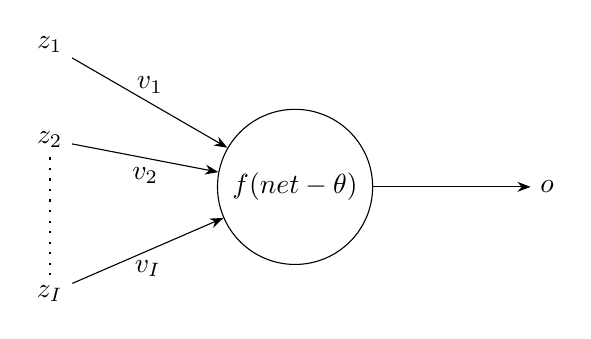
\begin{tikzpicture}[
  mycircle/.style={
     circle,
     draw=black,
     fill=white,
     inner sep=4pt,
     minimum size=20pt},
  mylabel/.style={font=\bf},
  myarrow/.style={-Stealth},
  node distance=1.5cm and 2cm
  ]
  \node[mylabel] (z1) {$z_1$};
  \node[mylabel,below=0.75cm of z1] (z2) {$z_2$};
  \node[mylabel,below=0.25cm of z2] (z3) { };
  \node[mylabel,below=1cm of z3]    (zn) {$z_I$};

  % neuron and output
  \node[mycircle, right=of z3] (neuron) {$f(net - \theta)$};
  \node[mylabel,  right=of neuron] (out) {$o$};

% edges
\draw [myarrow] (z1) -- node[above] {$v_1$} (neuron);
\draw [myarrow] (z2) -- node[below] {$v_2$} (neuron);
\draw [myarrow] (zn) -- node[below] {$v_I$} (neuron);

\draw [myarrow] (neuron) -- node[sloped] {} (out);

\path[] (z2) edge[thick, dash pattern=on \pgflinewidth off 3pt] node[] {} (zn);

\end{tikzpicture}
\caption{A NN which receives the inputs $z_1, z_2, ..., z_I$ and connects them to the neuron through the weighted edges $v_1, v_2, .., v_I$. The input values are multiplied by their respective weights and subtracted from a threshold ($\theta$). The result is passed to an activation function which produces the output \cite{Engelbrecht}.}
\end{figure}

% What is an activation?
% Define ReLU
An activation function computes a weighted sum of its input, adds a bias and decides whether the neuron's value should be propagated or not. A common choice for an activation function is the Rectified Linear Unit (ReLU) \cite{Relu}. A ReLU is defined as: $\sigma(x) = \max(0, x)$, where $x$ is the weighted sum of the inputs. It returns an output $x$ if $\sigma(x)$ is positive, $0$ otherwise. NN's using primarily ReLU activation functions have been shown to enable faster training even with many layers \cite{cnn-star-galaxy}.

\begin{figure}\label{fig:relu}
\centering
\begin{tikzpicture}[y=.4cm, x=0.4cm]
  %axes
  \draw [<->] (-10,0) -- coordinate (x axis mid) (10,0);
  \draw [->]  (0,0) -- coordinate (y axis mid) (0,10);

  %ticks
  \foreach \x in {-8,-6,...,8}
    \draw (\x,1pt) -- (\x,-3pt)
    node[anchor=north] {\x};

  \foreach \y in {2,4,...,8}
    \draw (1pt,\y) -- (-3pt,\y)
      node[anchor=east] {\y};

  % line
  \draw[blue] (-10,0) -- coordinate (x axis mid) (0,0);
  \draw[blue,thick, ->] (0,0) -- coordinate (y axis mid)(10,10);
\end{tikzpicture}
\caption{A ReLU function \cite{reluimage}.}
\end{figure}

It is possible for ReLU to introduce dead neurons whose output is always zero, this problem is known as the dying ReLU problem. To mitigate this issue, a slightly different version of ReLU known as leaky ReLU can be used. Leaky ReLU is defined in equation \ref{leaky-relu}.

\begin{equation}
\sigma(x) =
\begin{cases} \label{leaky-relu}
    x      , & \text{if } x\geq 0\\
    0.01x , & \text{otherwise}
\end{cases}
\end{equation}

Difference between the actual and predicted output (the error) is computed by loss function. In a NN, a loss function is used to correct weights after a feed forward operation, this process of correction is called back propagation. The error is propagated backwards from the output layer through the hidden layers to the input layer, wherein the weights and biases are modified in such a way that the error for the most recent input is minimized. Over many training samples the loss function will minimize error and the value of the weights for the whole network will begin to converge. The curve which the error rate of the network experiences is controlled through a gradient descent method. This method can help determine whether the network should be trained further or to stop early.

% TODO: more about gradient descent and early stopping, mention local minima

\subsection{Deep Learning}
% What is deep learning?
Deep learning is a set of algorithms in machine learning that attempt to learn in multiple levels, corresponding to different levels of abstraction. It is based on learning several levels of representations, corresponding to a hierarchy of features, where higher-level concepts are defined from lower-level ones, and the same lower level concepts can help to define many higher-level concepts. It typically uses artificial neural networks. An observation (e.g., an image) can be represented in many ways (e.g., a vector of pixels), but some representations make it easier to learn tasks of interest through examples (e.g., is this the image of a human face?). Research in this area attempts to define what makes better representations and the best methods for a NN to approach learning them \cite{DeepLearning}.

\subsection{CNNs}

% What is a CNN?
% What was it inspired by?
% When was this architecture created?
A CNN is a type of deep feed-forward neural network~\cite{cnn-star-galaxy} which is able to extract elementary visual features from its input. The creation of CNNs was motivated by Hubel and Wiesel's discovery in~\cite{hubel-wiesel-receptive-fields}, where they were able to find that a cat's visual cortex has locally sensitive, orientation-selective neurons. CNNs were first introduced in \citeyear{Lecun99objectrecognition} \cite{Lecun99objectrecognition}, and since then have been applied to solve numerous different type of problems in  natural language processing \cite{Collobert:2008:UAN:1390156.1390177}, image recognition \cite{cnn-star-galaxy}, and recommendation systems \cite{NIPS2013_5004}.

% What is the input of CNN?
% What is a convolution?
% What are CNNs made of?
% What are convolutional layers?
% What are filters?
% What are feature maps?
A CNN takes an image as an input and feeds it through several layers; usually convolutional layers with ReLU activation functions, pooling layers, and a fully-connected layer (FCL). Convolutions are the primary operation of a CNN and what makes them distinct from other type of networks. A convolutional layer parameters is made up of a set of small learnable weights known as filters. A filter has a local receptive field, and given an image as an input to a convolutional layer, it convolves each filter across the image's width and height using a specified stride size and produces outputs called feature maps \cite{cnn-star-galaxy}. Filters are what allow a CNN to learn to extract visual clues from its input such as edges, lines, and corners \cite{Lecun99objectrecognition}. Equation \ref{cnn:feature-map} from \cite{cnn-star-galaxy} gives the mathematical definition of a feature map $k$. The summation is performed over the set of input feature maps, the symbol $*$ describes the convolution operator, and $\boldsymbol{x}_m$ the filters.

\begin{equation} \label{cnn:feature-map}
y^k = \sigma{\bigg(\sum_{m} \boldsymbol{w}^{k}_{m} * \boldsymbol{x}_m + b^k \bigg)}
\end{equation}

% Why ReLU as activation functions?
The filters of a CNN compute linear element-wise multiplication and additions to create the feature maps. In order to add non-linearity, it is common for the convolutional layers to use ReLUs as the activation function which additionally allow for faster training in networks with many layers \cite{cnn-star-galaxy}.

% What is a pooling layer?
% How does a pooling layer work?
% How does a CNN reduce dimensionality?
Feature maps are then fed through pooling layers. A pooling layer is typically of size~$2 \times 2$~\cite{NIPS2012_4824}, and  its job is to essentially reduce the resolution of the previous feature map. A pooling layer performs an operation such as selecting the maximum value within its range, thus acting as a regularization technique to avoid overfitting.

% Why a fully-connected layer?
Finally, convolutional and pooling layers are followed up by a FCL. The FCL size needs to be the same as the number of classes or outputs the network has to learn to identify~\cite{Ciresan11flexible}, and its goal is to simply act as a classification layer which outputs the probability for each class.

% How are CNNs trained?
Once the architecture of a CNN has been specified, its filters and weights are initialized to small random values. Next, given an image as an input, it is fed through the convolutional, pooling operations, and the FCL. The output probabilities of the network are then used to compute the total error, and finally gradient descent is used to update the filter and weight values with respect to their contribution to the total error. This process is repeated with other images in the dataset until satisfactory results are achieved.

\section{Implementation}

% Data pre-processing, CNN setup, training, test, overfitting, data augmentation...

\subsection{Data Preprocessing}

All images in the dataset are of size $424\times424$ and the object of interest is always centered. In order to reduce the dimensionality of the images, during preprocessing images are cropped to $212\times212$, half their original size, images are also down sampled to half size again $ 106\times 106$, discarding unnecessary information in each image which could impair the network. Down sampling can help the CNN learn which regions are related to each specific expression as well as improve performance when training \cite{deep-learning-review}.
% data augmentation, cropping & downsampling => dimensionality reduction

\subsubsection{Data Augmentation}
While there are a sufficient count images to train on, it is possible to increase the performance of the network by augmenting the training data. Because the galaxies are rotationally invariant this dataset is an ideal candidate for applying data augmentation to. Therefore, a random transformation was performed online to different images across epochs. This transformation could be any combination of rotation by 90 degree increments or a flip on the horizontal or vertical axes, or no transformation at all (1 in 4 that there is no rotation, and 1 in four that there is no rotation at all). This brings 16 possible configurations for each image. Trained over 50 epochs there is a good likelihood that the network will see every configuration of any given image.

\subsection{CNN Architecture - VGG16}

\newcommand{\anet}{AlexNet\xspace}
\newcommand{\gnet}{GoogLeNet\xspace}
\newcommand{\inet}{ImageNet\xspace}

VGG-16 is a 16 weight-layer convolutional neural network used for image recognition. Created by the visual geometry group at Oxford in \citeyear{vgg16-arxiv} VGG-16 got second place to Google's \gnet in the Large Scale Visual Recognition Challenge (ILSVRC) 2014 \cite{vgg16-arxiv}. With the trained model released to the public, it is possible to build on top of the weights that are already set by the initial training phase. The advantage behind this is that the model doesn't need to be trained from scratch, this is a form of transfer learning. VGG-16 was trained on 1000 categories of images (classes).

Other pre-trained CNN architectures exist such as \gnet and \anet. \gnet uses average pooling instead of fully connected layers \cite{googlenet-paper} and beat VGG with an error rate of 6.67\% over VGG's 6.8\%. \anet won ILSVRC in 2012 and was novel for stacking multiple convolutional (conv) layers in a row before pooling their results \cite{alexnet-paper}. % so why is VGG advantageous again?

VGG is a clear choice over \gnet and \anet because the weights from the competition are available to the public for use and \anet and \gnet are not as readily available. Furthermore, VGG's fully connected nature without any special layers and widgets like \anet or \gnet make implementation and management much more simple. % hypothesis

\begin{table}
    \begin{center}
        \begin{tabular}{| c |}
        \hline
        Input $224 \times 224$ \\
        \hline
        Conv3-64 \\
        Conv3-64 \\
        \hline
        maxpool\\
        \hline
        Conv3-128 \\
        Conv3-128 \\
        \hline
        maxpool \\
        \hline
        Conv3-256 \\
        Conv3-256 \\
        Conv3-256 \\
        \hline
        maxpool \\
        \hline
        Conv3-512 \\
        Conv3-512 \\
        Conv3-512 \\
        \hline
        maxpool \\
        \hline
        Conv3-512 \\
        Conv3-512 \\
        Conv3-512 \\
        \hline
        maxpool\\
        \hline
        FC 4096\\
        \hline
        FC 4096\\
        \hline
        FC 1000\\
        \hline
        soft-max output\\
        \hline
        \end{tabular}
        \caption{VGG-16 architecture, a line between each item represents a weighted layer of which there are 16. VGG also made 11, 13,and 19 weight-layer variants which use different counts of convolutional layers \cite{vgg16-arxiv}.}
    \end{center}
\end{table}

% pooling sizes
% convolution sizes
% advantages over AlexNet, and ImageNet

% Architecture changes we have to make
While VGG-16 was trained on 1000 categories of images (classes), the Galaxy Zoo dataset has an expected output dimensionality of 37. Therefore, several changes had to be made to the network architecture to support the inputs and ouputs of our experiments. The last layer is set to 37 neurons. On the input layer of VGG-16, because the preprocessing methods crop and down-sample from $424 \times 424$ pixels to $106 \times 106$ pixels the input layer needs to be one of size $3 \times 106 \times 106$ (three because the images have three color channels: red, green, blue). Another change made for this problem was changing the output layer activation function from soft-max to sigmoid. With this new network architecture the pre-trained weights from the ILSVRC competition released to the public by VGG were unusable, this meant training from scratch was necessary. Fortunately the hardware to do such training was available (see \ref{hard-soft-ware}).

\subsection{Dropout}
Dropout is a method to prevent neural networks from overfitting \cite{dropout}. It does this by randomly deactivating some neurons in one --or many-- layers. This makes the remaining active neurons compensate their weights twice as much in the back-propagation phase. Neurons are randomly activated and deactivated per update; here, each time a batch has been fully fed through the network. By activating and deactivating neurons in layers, dropout keeps the neurons of a network robust to the training data by never letting them fully fit to the training data. In \cite{dropout} the authors recommend to keep dropout ratio between $0.5$ and $1$. In the implementation of VGG-16 we stuck with the 50\% dropout rate which the original implementors chose. In this VGG-16 implementation dropout only applies to the final two FCL layers. This means that during any given batch only 2048 neurons are actually active in each layer.

\subsection{Hyperparameters}

% learning rate, activation functions, rprop optimization method, batch sizes.
We adopted a learning rate of $10e-6$ from the original VGG paper.

Early validation splits were very high, at 95\% training and 5\% validation (95/5) this split was producing models which were overfit as evidenced by poor performance as well as the training loss on the model becoming --sometimes significantly-- less than the validation loss. Later, this was changed to a more traditional validation split of 80/20.

%Batch sizes 16 and 32.
Dimensions of the images can be reduced dramatically and still be useful to the network. Two image sizes were tried, $106 \times 106$ and $69 \times 69$. Different batch sizes were tried too: 16, 32. These batch sizes determine how fast the weights of the network get updated. The smaller the batches get to one the closer the network gets to using simple gradient descent methods. Because our dataset and the number of parameters in the network are both large, adjusting weights with an extreme frequency could lead to getting stuck in minima or over-adjusting and missing our target function.

Another change from the presented VGG-16 implementation was the output layer activation function. We chose sigmoid over soft-max, this was an important change because the soft-max function has difficulty predicting hard zeros and ones \cite{kaggle-winner}. Throughout the dataset there are many hard zero values which represent the galaxy not having that attribute at all.

\subsection{Software and Hardware}\label{hard-soft-ware}
For the software implementations there are two readily available and widely used machine learning frameworks Keras and TensorFlow. Keras is a high-level machine learning library written in Python. It can be used with a range of backend drivers which makes it very portable. TensorFlow is the backend driver we used with Keras which allows access low level hardware for training.

A NVidia GeForce 970 graphics processing unit (GPU) was available, it was used for training each of the models described in results section. GPU's allow for embarrassingly parallel computations and neural networks can be placed in that domain of being embarrassingly parallel. Using a GPU decreased training time by an order of magnitude over traditional CPU's.

\section{Results}

%"We don't care much about results, except when they're bad." - Ölle

% save me I'm useful somewhere
% \begin{equation}\label{rmse}
% RMSE(y,\hat{y}) = \sqrt{\frac{1}{n}  \sum_{i=1}^{n} (y_i - \hat{y}_i)}
% \end{equation}

Each model was trained for at most fifty epochs on the full training dataset. Early runs were trained with a 90/10 training-validation split, there didn't seem to be much room for improvement based on the separation between the validation and training loss (figure \ref{32b-106-90-10}). Thus, an 80/20 split was settled on. Early stopping would be invoked if validation loss did not improve for five epochs. To make sure the results could be equally quantified the dataset was shuffled with the same random seed each time.

\subsection{Benchmarks}\label{benchmarks}
The Galaxy Zoo Kaggle competition has a test image set of \numprint{79975} images. After training the model the network uses these images to produce predictions. These predictions are saved as a CSV file and uploaded to Kaggle. Kaggle then scores the predictions using the root mean square error (RMSE) between the model predictions and what the actual values are, (these actual values for the test set are kept secret) the lower scores are better. There are certain basic thresholds which can be used to determine if your model behaves as a random classifier or worse. The first is an All Zeros benchmark, this is equivalent to a network that always outputs zeros for all attributes. Similarly, there is an All Ones benchmark; these two benchmarks represent random classifications which, while not entirely trivial to pass, require some rational architectural choices. The final benchmark is harder, a Central Pixel benchmark, which are the predictions if the outputs were simply the central pixel RGB value in each training image. Very early implementations of the VGG16 model could pass the All Zero benchmark, later--with the right hyper-parameters-- the model could pass the All Ones and Central Pixel benchmarks. Results through the rest of this paper are based on the RMSE score Kaggle given for a particular model.

\subsection{Performance}

Before immediately attempting data-augmentation methods, a few hyperparameter configurations were run to get a better idea of the best input size and the best batch size for moving forward.

\begin{table}[]
    \centering
    \begin{tabular}{|r|c|c|}
        \hline
                      & \isize{69} & \isize{106} \\ \hline
        Batches of 16 & 0.11538 & 0.11062 \\ \hline
        Batches of 32 & 0.11476 & 0.11288 \\ \hline
    \end{tabular}
    \caption{Spread of results for various input and batch sizes. In the Kaggle competition this would put us in 78, 88, 94, 95 place respectively.}
    \label{tab:results1}
\end{table}

Results for the images were \isize{69} and where the batch size was 32 or 16 the loss graph and validation loss exhibited traits of overfitting (figure \ref{32b-69}). The results from Kaggle may in fact back this up, as the score gets better the larger the batch size, although two points don't necessarily make a trend. It could be that larger batch sizes may be necessary when the images are smaller.

\pngfigure{32b-69}{The training loss line being lower than the validation loss line characteristic of overfitting.}

\pngfigure{32b-106-90-10}{A run with a 90/10 training-validation split, the score from this run was admissible but ultimately beat by 80/20 splits.}

% This figure feels a little redundant
\pngfigure{32b-106-80-20}{A run with 80/20 training-validation split. Notice the smoother curve versus a run with the same parameters but a 90/10 split.}

\subsection{HSV Input format}

In digital imagery pixels are stored as combinations of three values red, green, and blue (RGB). However, there are many more ways to represent color; in printing for example: cyan, magenta, black (CMYK) are optimal values because of how light reflects on printed surfaces. Hue, saturation, value (HSV) is a different color space where the color is stored in hue, color intensity is stored in saturation, and the brightness is stored in a value. There were hypothesis if converting the galaxy images to this color format might enhance responses in the network, stars being bright, the star pixels will emit a high $V$ value and thus create stronger weights.

The results from this color space conversion were not terrific. With a batch of 32 with images the image size of \isize{106} got a score of $0.13778$ worse than any RGB result. The score was worse due to two issues over which there was much rumination. While $V$ may have been regularly high for the features we're trying to detect, $H$ may have been too varied for the network to converge on. For $S$, the color intensity of images was not very high, and so most colors were close to zero on the saturation scale. The combination of a rapidly fluctuating variable $H$, a regularly small value of $S$ made $V$ comparatively worthless to the network. This score would have earned 178^{th} in the Kaggle competition.

\subsection{Data Augmentation}
After the examining the results on 32 and 16 batches we decided to move forward with applying data augmentation to image sizes of \isize{106}.

\begin{table}[]
    \centering
    \begin{tabular}{|r|c|}
        \hline
                      & \isize{106} \\ \hline
        Batches of 16 &  0.11331 \\ \hline % 91
        Batches of 32 &  0.11673 \\ \hline % 97
    \end{tabular}
    \caption{Spread of results for various batch sizes with data augmentation. Augmentation was a random combination of reflection on the horizontal or vertical axis and being rotated by 90 degree increments. }
    \label{tab:results2}
\end{table}

This reinforces a forming hypothesis that smaller batch sizes for the \isize{106} image sizes are more optimal. These scores would have earned 91st and 97th respectively. There may be too much augmentation going on and not enough hyperparameter adjustment. As section \ref{aug} mentions, there are almost a million images with these transformations, it might have been best to perform some learning rate studies, for as is, the network might not have taken the large strides it needed to to get a better score than the un-augmented datasets.
\section{Conclusion}

Summarize your contributions


\bibliographystyle{plainnat}
\bibliography{references}
\end{document}
